
Outline:

- Motivace
- Co je responzivní design
- Responzivní design v LaTeXu
  - přizpůsobení velikosti fontu velikosti zobrazení
  - typografická stupnice
  - media queries
    - změny počtu znaků na řádek
    - okraje pomocí newgeometry
- Automatizovaná sazba
  - luvlna
  - luawidowcontrol
    - každý odstavec sází dvakrát -- jeden s normálními parametry, druhý o jeden řádek větší
    - pokud se najde parchant, vymění předešlý odstavec za verzi s rádkem navíc
    - nastavení:
 \begin{verbatim}
 \lwcsetup{⟨preset⟩}
 \end{verbatim}
      - default - nepřidává žádné vertikální mezery, ale může vést k příliš vzdušným odstavcům
      - strict - využívá primárně vertikální mezery a nevytváří špatné odstavce,  ale odstraní jen třetinu parchantů
      - balanced - kombinuje obě metody, odstraní 90\% parchantů
    - upozornění:
      - \verb|\clubpenalty| a \verb|\widowpenalty| nemají žádný efekt, naopak mohou způsobit vedlejší účinky
      - podpora pro více sloupcovou sazbu je omezená, balíček Multicol nefunguje
  - linebreaker

 
\begin{frame}
  \frametitle{Porovnání různých metod k omezení parchantů}
  \begin{center}
  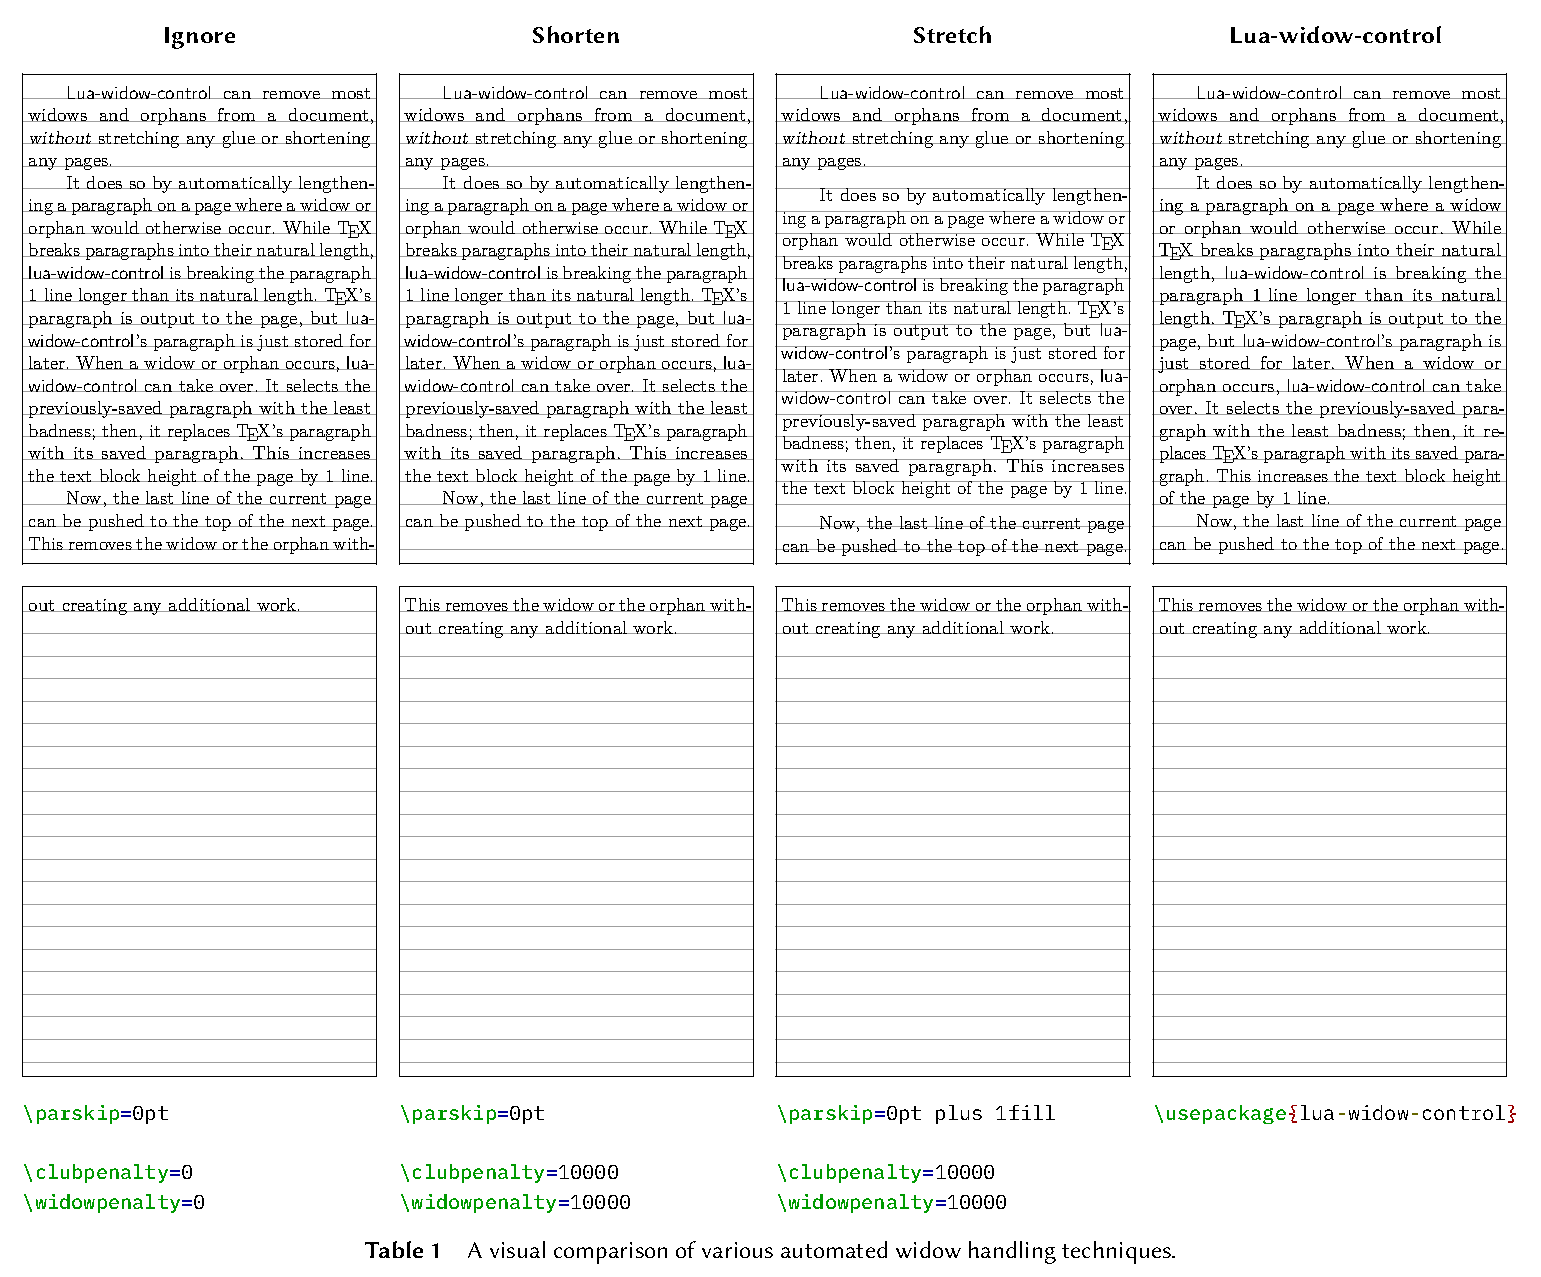
\includegraphics[height=.95\textheight]{img/lua-widow.pdf}
  \end{center}
  % \myfig[height=0.8\textheight]{img/lua-widow.pdf}{}
\end{frame}



\begin{frame}
  \frametitle{How are hooks configured}
  \begin{itemize}

\end{itemize}
\end{frame}

\begin{frame}[fragile]
  \frametitle{\texttt{tex4ht.sty} package options}
  \begin{priklad}
\begin{verbatim}
$ make4ht filename.tex "mathml,mathjax"
\end{verbatim}
\end{priklad}
\end{frame}
